\chapter{Quantum Cryptography}%
\label{cha:Quantum Cryptography}

\section{Quantum Key Distribution}

This section is about quantum key distribution (QKD) protocol of Bennet and Brassard 1984 (BB84) for the \important{generation of common one-time pad shared by two distant parties Alice and Bob}.
\begin{parag}{One-time pads}
    This is a sequence of secret bits $z_1, z_2, \ldots, z_m$, $z_i \in \left\{0, 1\right\}$ shared by Alice and Bob (which are supposed to be at two distant locations). It is used as follows:
	\begin{itemize}
	    \item If Alice has a message $m_1m_2\ldots m_M$ to communicate, she encodes it as 
			\begin{align*} 
				\left(z_1 \oplus m_1\right)\left(z_2 \oplus m_2\right)\ldots \left(z_M \oplus m_M\right)
			\end{align*}
			and sends the sequence to Bob. Then Bob can decode it as 
			\begin{align*} 
				\left(z_i \oplus m_i\right) \oplus z_i = m_1 
			\end{align*}
			This scheme of encrypting is theoretically a secure scheme if the one-time pad is i.i.d. (independent identically distributed) uniformly random and is used only once.
			\item The trouble is how to distribute it to Alice and Bob and make sure it is not intercepted
	\end{itemize}
\end{parag}
\begin{center}
    The point of the QKD is that we do not distribute the one-time pad but generate it directly in the labs of Alice and Bob.
\end{center}


\subsection{BB84 protocol for QKD}
Here let us review the main phases of the protocol
\begin{enumerate}
    \item Encoding phase of Alice
    \item Decoding phase of Bob
    \item Public communication phase of Alice and Bob
    \item Generation of common secret bit sequence and the '\textit{security check}'
\end{enumerate}
Finally, we will review some possible attacks from eavesdroppers and argue whether the protocol is secure.

\begin{parag}{1: Encoding in Alice's lab}
    \begin{itemize}
        \item Alice generates two uniformly random i.i.d. sequences of classical bits 
			\begin{align*} 
				x_1 x_2 \ldots x_N \in \left\{0, 1\right\}^{N}\\
				e_1 e_2 \ldots e_N \in \left\{0, 1\right\}^{N} \mathspace\text{ secret for the moment}
			\end{align*}
			\item For $e_i = 0$ Alice prepares a qbit $\ket{x_i} \in \left\{\ket{0}, \ket{1}\right\}$ (in the computational basis)
			\item For $e_i = 1$, Alice prepares a qbit 
				\begin{align*} 
					H\ket{x_i} \in \left\{\frac{\ket{0} + \ket{1}}{\sqrt{2}}, \frac{\ket{0} - \ket{1}}{\sqrt{2}}\right\} 
				\end{align*}
				In the Hadamard basis $H = \frac{1}{\sqrt{2}}\begin{pmatrix} 1 & 1 \\ 1 & -1 \end{pmatrix} $
    \end{itemize}
	\begin{framedremark}
	Physically you can think about polarized states of photons for the qbits.
	\end{framedremark}
	To summarize, at each instant $i= 1, \ldots, N$ Alice has prepared a qbit in the state 
	\begin{align*} 
		H^{e_i}\ket{x_i} 
	\end{align*}
	\begin{subparag}{Remark}
	    The power here $e_i \in \left\{0, 1\right\}$ just say if $e_i = 1$ then apply $H$, which just a notation trick.
	\end{subparag}
	Hence we have that the qbits we are sending are inside the set 
	\begin{align*} 
		H^{e_i}\ket{x_i} \in \left\{\ket{0}, \ket{1}, \frac{\ket{0} + \ket{1}}{\sqrt{2}}, \frac{\ket{0} - \ket{1}}{\sqrt{2}}\right\} 
	\end{align*}
	A then sends this qbit to Bob through a quantum channel (optic fibers, free space etc.)
\end{parag}

\begin{parag}{Decoding in Bob's lab}
    Bob receives the qbit (photon polarization) for each $i= 1, \ldots, N$. He has no idea of the state. He does a measurement at each instant.
	\begin{itemize}
	    \item Bob generates an i.i.d. uniformly random sequence of bits 
			\begin{align*} 
				d_1 d_2 \ldots d_N \in \left\{0, 1\right\}^{N}
			\end{align*}
			\item For $d_i = 0$ he choose the measurement basis $\left\{\ket{0}, \ket{1}\right\}$ to do his measurement
			\item For $d_i = 1$ he choose the measurement basis $\left\{\frac{\ket{0} + \ket{1}}{\sqrt{2}}, \frac{\ket{0} - \ket{1}}{\sqrt{2}}\right\}$
	\end{itemize}
	In summary, his output state is $H^{d_i}\ket{y_i}$
\end{parag}
\begin{parag}{3: Public communication phase}
    Now Alice and Bob share publically their encoding and decoding sequences $e_1, \ldots e_N$ and $d_1, \ldots d_N$. Anybody may know these sequences. However $x_1, \ldots, x_N$ and $y_1, \ldots, y_N$ are \important{not} revealed
\end{parag}
\begin{parag}{4: Generation of one-time pad}
    \begin{itemize}
        \item If $e_i = d_i$, Alice and Bob keep the bits $x_i$ and $y_i$. It turns out that $x_i = y_i$
        \item If $e_1 \neq d_i$, then Alice and Bob discard the bits $x_i$ and $y_i$. It turns out thats those may be different or equal
    \end{itemize}
	\begin{subparag}{Security check}
	    out of $i = 1\ldots N$ such that $e_i = d_i$ Alice and Bob select $\frac{\epsilon N}{2}$ such instances ($0 < \epsilon \ll 1$) and sacrifice the $\left(x_i, y_i\right)$ by echanging then on the public channel. Thus they check if indeed $x_i = y_i$. If this let passes they conclude that the protocol has worked well and nobody has been eavesdropping.\\
		Essentially the security check lets if 
		\begin{align*} 
			\frac{1}{\left(\frac{\epsilon N}{2}\right)} # \left\{i \in \left[\frac{\epsilon N}{2}\right] \subset \left\{1, \ldots, N\right\}\mathspace  \text{ s.t. } e_i =  d_i \mid x_i = y_i\right\}  \approx 1
		\end{align*}
		Remark that here the noise of the channel should be specified and low enough so that we are able to distinguish noise from eavesdroppers.
	\end{subparag}
\end{parag}

\begin{parag}{Lemma}
    This whole protocol is justified by the following lemma:
	\begin{align*} 
		\begin{cases}
			P\left(x_i = y_i | e_i = d_i\right) = 1\\
			P(x_i \neq y_i | e_i = d_i)= 0
		\end{cases}   \\
		\begin{cases}
			P\left(x_i = y_i | e_i \neq d_i\right)  = \frac{1}{2}\\
			P\left(x_i \neq y_i | e_i \neq d_i\right) = \frac{1}{2}
		\end{cases} 
	\end{align*}
\end{parag}
\begin{parag}{Proof}
    Let us compute the first point of the first case $P\left(x_i = y_i | e_i = d_i\right)$. Here we can separate it into two cases
	\begin{align*} 
		P\left(x_i = y_i | e_i = d_i\right) &= P\left(x_i = 0, y_i = 0| e_i= d_i\right) + P\left(x_i = 1, y_1 = 1| e_i = d_i\right) \\
											&=  P\left(y_i = 0| x_i = 0, e_i = d_i\right)P\left(x_i = 0\right) + P\left(y_i = 1| x_i = 1, e_i = d_i\right)P\left(x_i= 1\right)
	\end{align*}
	Then using Bayes law we have $P\left(A|B\right) = \frac{P\left(A \cap B\right)}{B} \implies P\left(A \cap B\right) = P\left(A|B\right) P\left(B\right)$. Now what is the state given to Bob when $x_i = 0$? It is $H^{e_i}\ket{0}$. If $e_i = 0$ then we have sent $\ket{0}$ which as $d_i = e_i = 0$ Bob will measure using the basis $\left\{\ket{0}, \ket{1}\right\}$ output $y_i = 0$ with probability 1. On the other side if $e_i = d_i = 1$ then Alice will have sent $\ket{+}$ and Bob will measure it using the basis $\left\{\ket{+}, \ket{-}\right\}$ which will also output $y_i = 0$ with probability 1. The same measurement can be done when $y_i = 1$ giving 
	\begin{align*} 
		P\left(x_i = y_i | e_i = d_i\right) &= P\left(x_i = 0\right) + P\left(x_i = 1\right) \\
											&= \frac{1}{2} + \frac{1}{2} = 1
	\end{align*}
	Hence $P\left(x_i \neq y_i|e_i = d_i\right) =  1 - P\left(x_i = y_i |e_i = d_i\right) = 0$.\\
	$ $\\
	Let us now look at the other case 
	\begin{align*} 
		P\left(x_i = y_i | e_i \neq d_i\right) &= P\left(x_i = 0, y_i = 0| e_i \neq d_i\right) + P\left(x_i = 1, y_i =1| e_i \neq d_i\right)\\
											   &= P\left(y_i = 0| e_i \neq d_1, x_i = 0\right)P\left(x_i = 0\right) + P\left(y_i = 1| e_i \neq d_i, x_i = 1\right)P\left(x_i = 1\right)\\
	\end{align*}
	If $e_i \neq d_i$, we have that the state sent to Bob is on the other basis that the one it will be measured with. Meaning that if the state sent is $\ket{0}$ then it will be measured with the $\left\{\ket{+}, \ket{-}\right\}$ basis hence the probability of having $y_i = 0$ is given as 
	\begin{align*} 
		\left|\bra{+}\ket{0}\right|^2 &= \frac{1}{2}
	\end{align*}
	Now if the state sent is $\ket{+}$ which implies that $e_i = 1$ then $d_i = 0$ which therefore mean that we will measure using the basis $\left\{\ket{0}, \ket{1}\right\}$ hence giving the probability that $y_i = 0$ as 
	\begin{align*} 
		\left|\bra{0}\ket{+}\right|^2 = \frac{1}{2}
	\end{align*}
	Which implies that $P\left(y_i = 0| e_1 \neq d_i, x_i = 0\right) = \frac{1}{2}$ and the same goes for the $y_i = 1$ case giving 
	\begin{align*} 
		P\left(y_i = y_i | e_i \neq d_i\right) = \frac{1}{2} \frac{1}{2} + \frac{1}{2} \frac{1}{2} = \frac{1}{2}
	\end{align*}
\end{parag}

\subsection{Attack from an eavesdropper}
A complete discussion of security of the scheme goes well beyond this course. One must imagine that an eavesdropper captures photon on the quantum channel, process them (with unitary evolutions and measurements), sends them back to Bob etc. The space of possible attack is huge and here we just scratch the surface of this subject by analyzing a very simple type of attack.
\begin{figure}[h!]
\centering
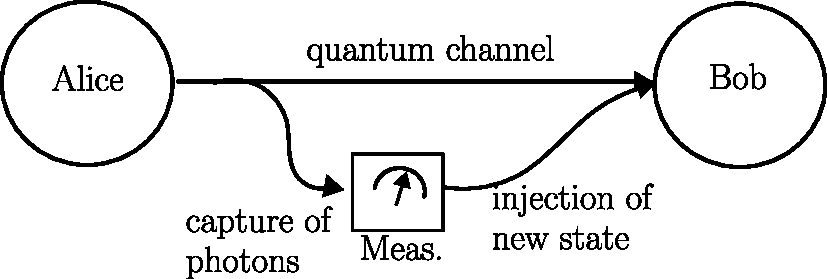
\includegraphics[width=0.6\textwidth]{figure/2026-10-22_3.pdf}
\caption{Setup of the eavesdropper attack}
\end{figure}


\begin{parag}{Measurement attack}
    Let us imagine the following setup 
	\begin{itemize}
	    \item Eve captures photons in state $H^{e_i}\ket{x_i}$
	    \item Measures in computational or Hadamard basis according to a random sequence she generates
			\begin{align*} 
				E_1 E_2 \ldots E_N \in \left\{0, 1\right\}^{N}
			\end{align*}
			Note that she has no idea of $e_i, d_i$ before public communication phase.
			\item The measurement learn the photon in state 
				\begin{align*} 
					H^{E_i} \ket{y_i^{\text{Eve}}} \mathspace ; y_i^{\text{Eve}} \in \left\{0, 1\right\}
				\end{align*}
				\item The state $H^{E_i}\ket{y_i}^{\text{Eve}}$ is forwarded to Bob.
				\item Bob measures as usual (he doesn't know what happens on the quantum channel) and he gets a state $H^{d_i}\ket{y_i}$ as before but this time with probability 
					\begin{align*} 
						\left|\bra{y_i}H^{d_i}H^{E_i}\ket{y_i^{\text{Eve}}}\right|^2
					\end{align*}
	\end{itemize}
	We now have the following lemma 
\end{parag}
\begin{parag}{Lemma}
    \begin{align*} 
    	\begin{cases}
			P_{\text{Eve}}\left(x_i = y_i| e_i = d_i\right) &= \frac{3}{4}\\
			P_{\text{Eve}}\left(x_i \neq y_i| e_i = d_i\right) = \frac{1}{4}
    	\end{cases}  
    \end{align*}
	Where $P_{\text{Eve}}$ mean the probability calculated in presence of Eve as in the sense of the probability of the decoding being '\textit{right}' For Alice and Bob when Eve is disturbing everything.\\
	$ $\\
	This lemma implies that the security protocols is not passed \important{after} the public communication phase since $\frac{1}{4}$ of potential one-time-pad is corrupted:
	\begin{align*} 
		\frac{1}{\frac{\epsilon N}{2}} # \left\{i \in \left[\frac{\epsilon N}{2} \subset \left[1, \ldots, N\right] \text{ s.t. } e_i = d_i| x_i = y_i\right]\right\}  \approx \frac{3}{4} < 1
	\end{align*}
\end{parag}
\begin{parag}{Proof}
    Now let us compute as before:
	\begin{align*} 
		P_{\text{Eve}}\left(x_i = y_i | e_i = d_i\right) &= P\left(x_i = y_i | e_i = d_i, E_i = e_i\right)P\left(E_i = e_i\right) + P\left(x_i = y_i| e_i = d_i, E_i \neq e_i\right) P\left(E_i \neq e_i\right)\\
	\end{align*}
	In the first case here we have '\textit{correctly guessed}' the state sent by Alice hence we resend the same state back to Bob giving that the probability of a good state is $1$. On the other hand we have incorrectly guessed the basis in which the state has been sent to Bob which therefore means that the state sent to Bob is in the wrong basis This implies that that probability is equivalent to 
	\begin{align*} 
		&= P\left(x_i = y_i| e_i = d_i\right) P\left(E_i = e_i\right) + P\left(x_i = y_i| e_i \neq d_i\right) P\left(E_i \neq e_i\right)\\
	\end{align*}
	A more formal way than before to compute the first term here is using Born rule on the state sent to Bob and the eigenvector of the measurement 
	\begin{align*} 
		P\left(x_i = y_i| e_i = d_i, E_i = e_i\right) &=  P\left(y_i^{\text{Eve}} = y_i | E_i = d_i\right)\\&= \left|\bra{y_i}\underbrace{H^{d_i}H^{E_i}}_{= I}\ket{y_i^{\text{Eve}}}\right|^2\\
													  &= \left|\braket{y_i}{y_i^{\text{Eve}}}\right|^2 = 1
	\end{align*}
	On the right hand side given $E_i \neq e_i$ we have $y_i^{\text{Eve}}= x_i$ with probability $\frac{1}{2}$ Thus 
	\begin{align*} 
		P\left(x_i = y_i |e_i = d_i, E_i \neq e_i\right) &= P\left(\right) 
	\end{align*}
\end{parag}
The question that this is raising is what does Eve wins other than disturbing Bob's and Alice's key?\\
$ $\\
Recall that the attack can be stated as follow, Eve takes the qbits from Alice and does a random measurement on them, and send the resulting state to Bob, therefore after Alice and Bob have shared they bit sequences, she know exactly the state sent to Bob and also $d_i$ and $e_i$ hence when $d_i$ matches $E_i$ Eve have access with certainty the bit that Bob has decoded As the probability is computed as 
\begin{align*} 
	\left|\bra{y_i}\underbrace{H^{d_i}H^{E_i}}_{= I}\ket{y_i^{\text{Eve}}}\right|^2 = 1
\end{align*}
If $e_i = d_i = E_i$ then Alice, Bob and Eve share the same bit with certainty. When $e_i = d_i \neq E_i$ then Eve knows that Bob has a resulting that is right with probability $\frac{1}{2}$. The reasoning can be done as follow:\\
As $e_i \neq E_i$ Eve measure with the wrong basis giving equal probability to both state sent to Bob. For instance if she receives $\ket{0}$ from Alice then with equal probability she will send $\ket{+}$ and $\ket{-}$ to Bob. As Bob as $e_i = d_i$ He will measure using the other basis that the one used by Eve hence having equally likely result for both outcome which implies that there is a probability $\frac{1}{2}$ of Bob having the wrong bits while thinking he has a matching one with Alice.
    

However this is already '\textit{good}' but this is not where Eve gains the most.  Recall what happens when $E_i = e_i$, in that case, Eve perfectly decodes the state and resend it back to Bob. If $d_i = e_i = E_i$ then all three share the bits with certainty which could be useful if there weren't $25 \%$ of errors.


\begin{parag}{Impossibility of '\textit{copy photon}' and resend attack}
    One could say here, well Eve could just  copy the qbit that she received, send one to Bob and measure on her. What this would require is that we have a machine which create a copy of a qbit based on another qbit. This machine can be represented as a unitary operator hence we would have
	\begin{align*} 
		U\left(\ket{\psi} \otimes \ket{\text{blank}}\right)  = \ket{\psi} \otimes \ket{\psi}
	\end{align*}
	Which if you have done homework 3 would know that this is not possible for $\ket{\psi}$ that are non orthogonal. And in fact here recall that our states can take all of the following values 
	\begin{align*} 
		\left\{\ket{0}, \ket{1}, \frac{\ket{0} + \ket{1}}{\sqrt{2}}, \frac{\ket{0} - \ket{1}}{\sqrt{2}}\right\} 
	\end{align*}
	Hence we are protected from copying by the no cloning theorem.
\end{parag}











 
